%!TEX root = ../thesis.tex
%*******************************************************************************
%****************************** Second Chapter *********************************
%*******************************************************************************

\chapter{Exploring the solution}

\section{Research on current implementations}

Companies like Amazon and Ocado have been at the forefront of technological advancement, deploying sophisticated robotic systems to improve efficiency, reduce costs, and enhance safety.

\begin{figure}[h!] 
\centering    
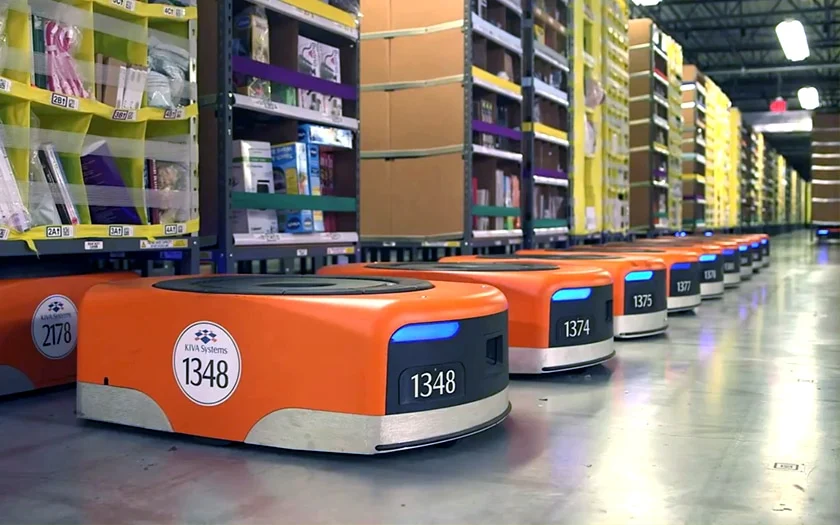
\includegraphics[width=0.8\textwidth]{Images/kiva.png}
\caption{- Amazon's robots \cite{amazonrobotics_2024_closeup}}
\label{robot}
\end{figure}

\subsection{History of warehouse robots}

The history of warehouse robotics is relatively recent. General Motors pioneered the field in 1961 by installing the first robotic arm, known as Unimate \cite{a2024_joseph}, to automate tasks in manufacturing. For several decades, warehouse robots weren't sophisticated enough to go beyond pre-programmed tasks. Around the 21st century, advances in computing power and sensors enabled robots to perform tasks with greater autonomy and independence. The development of real-time image recognition software and improvements in robotic movement eventually led to the creation of robots capable of navigating warehouse environments.

\newpage

\subsection{Amazon Robotics (formerly Kiva Systems)}

Amazon's robotics infrastructure is perhaps the most well-known large-scale implementation of automated warehouse management. Following Amazon's acquisition of Kiva Systems in 2012, the technology has been deployed across hundreds of fulfilment centres globally, with over 200,000 robots in operation as of 2020 \cite{edwards_2020_amazon}, with an average of 15,000 added each year to warehouses around the world. This figure will no doubt increase as investments in robotics and AI are part of the e-commerce giant’s \$100bn planned capital expenditure this year. \cite{clifford_2025_amazon}

\subsubsection{Centralised Control with Distributed Execution}
The system architecture employs a hierarchical control structure where high-level planning occurs centrally while individual robots maintain some autonomy for local decision-making. This hybrid approach enables the system to manage thousands of robots simultaneously while remaining responsive to local conditions. The central system breaks the warehouse floor into a grid of approximately 1 square meter cells, each uniquely identifiable through QR-code markers.

\subsubsection{Reservation-Based Traffic Management}
Rather than simply calculating shortest paths, the robots use reservation-based path planning, where robots not only find optimal routes but also reserve specific grid cells for specific time intervals, which prevents conflicts before they occur rather than relying solely on reactive collision avoidance. Each robot is aware of where they should be at exact times.

\subsubsection{Dynamic Re-slotting and Inventory Positioning}
The system continuously analyses product demand patterns and adjusts inventory positions to minimise average travel distances. Frequently ordered items move closer to packing stations, while seasonal or rarely ordered products move to other storage locations further away, meaning overall collection times are reduced.

\subsubsection{Multi-Objective Path Optimisation}
Amazon's robots consider multiple factors in their routing algorithms, including battery efficiency and charge status, task priority and delivery deadlines, current congestion patterns, predicted future congestion based on planned robot movements and historical traffic density data. This multi-objective optimisation reduces robot travel distance compared to standard shortest-path algorithms, significantly extending battery life and increasing system throughput.\newline
\textbf{ }
\newline While some of these features are beyond the scope of my project due to complexity, I believe a less advanced multi-objective path optimisation could be implemented into the A* algorithm as part of refinements to the program, dependent on performance and time remaining. \newline References: \cite{scallog_2024_amazon}

\subsection{Ocado Smart Platform: The Grid-Based Approach}

The Ocado Smart Platform (OSP) takes a fundamentally different approach to warehouse automation compared to Amazon's system, using a dense grid structure where robots move across the top of a storage grid rather than moving the storage units themselves.

\subsubsection{The Hive Mind Architecture}
Ocado's system uses a proprietary control system called "The Hive Mind", which coordinates hundreds of robots moving on a three-dimensional grid. The system uses a combination of centralised planning for global optimisation and edge computing for rapid local decisions. Each robot communicates with nearby robots multiple times per second to coordinate movements, while the central system performs broader optimisation at a lower frequency.

\subsubsection{4D Path Planning}
Similar to Amazon but a more sophisticated, robots reserve both physical slots as well as time — specific grid positions at specific moments. This allows robots to schedule crossings through the same physical space by assigning different time slots, meaning they have a greater number of robots at any one point.

\subsubsection{Swarm Behaviour Implementation}
While the system uses a central system for control, it also implements swarm principles; robots communicate with neighbouring units to form general patterns of movement that distribute across the grid faster. This approach allows the warehouse to gracefully degrade performance when components fail, rather than experiencing catastrophic failures due to a single failure. \newline
\textbf{ }
\newline While some of these implementations by Ocado are impressive, I do not believe I will be able to implement anything similar from this, other than the model of robots moving in a 2D space despite a 3D warehouse. Since Ocado store the same item vertically, I could apply the same principle to StockBot, reducing the need for 3D considerations, which would make my project much more complex and beyond the scope of my aim. \newline References: \cite{a2024_joseph}, \cite{group_2024_the}, \cite{group_2023_the}, \cite{group_2020_explained}

\subsection{AutoStore: Cube Storage}

AutoStore's approach to automated storage and retrieval is similar to Ocado, using a three-dimensional storage cube accessed by robots operating on the top surface. Ironically, they were in a 3-year legal battle with Ocado over the patents surrounding these robots, before settling to share the patent in a mutually beneficial agreement \cite{speed_2023_ocado}

\subsubsection{Cube Storage Efficiency}
The AutoStore system achieves remarkable storage density by eliminating aisles entirely. Bins are stacked directly on top of each other in a dense grid, with robots traversing the top surface and retrieving bins through vertical shafts. This approach achieves significantly higher storage density than traditional automated systems and conventional shelf storage.

\subsubsection{Grid-Based Robot Movement}
The robots move on an aluminium grid structure along straight paths, but with a unique feature; when two robots need to traverse the same grid space, one robot can physically drive on top of another, then continue its journey when the bottom robot moves to its destination.

\subsubsection{Bin Retrieval Algorithms}
The system employs sophisticated algorithms to determine which bins to retrieve and in what order, especially when a single order requires items from multiple bins:
\begin{enumerate}
    \item The system first establishes if multiple items from an order might be in the same bin.
    \item It then calculates the optimal sequence to retrieve bins, considering their vertical positions.
    \item Bins needed for imminent orders are often pre-positioned near the top of stacks.
    \item The algorithm continuously balances retrieval efficiency against grid traffic density.
\end{enumerate}

\subsubsection{Decentralised Control with Hierarchical Oversight}
Unlike Amazon's more centralised control, AutoStore employs a more distributed approach where individual robots have substantial influence in path selection. A central system provides high-level task allocation, but robots resolve movement conflicts directly with neighbouring units. References: \cite{autostore_2023_autostore}, \cite{solutions_2025_autostore}, \cite{systems_2018_autostore}, \cite{systems_autostore}

\newpage

\section{Research on pathfinding algorithms}

\subsection{Breadth-First Search (BFS)}
Breadth-First Search $^{\cite{point_data}}$ is an uninformed algorithm which begins at a specified start node and systematically explores all neighbouring nodes at the present depth level before moving to nodes at the next depth level. The boundary of this level is often referred to as the frontier. BFS maintains a queue of nodes to visit, implementing a first-in-first-out (FIFO) system that ensures all nodes at a given depth are processed before any nodes at a greater depth. This guarantees that when a goal node is discovered, the path to it will have traversed the minimum number of edges possible.
\subsubsection{Properties}
\begin{itemize}
    \item \textbf{Time Complexity:} The time complexity of BFS is $O(b^d)$, where $b$ represents the branching factor (the average number of successors per node) and $d$ represents the depth of the shallowest solution. In the worst case, BFS must explore all nodes up to the depth of the solution.
    
    \item \textbf{Space Complexity:} Space complexity is also $O(b^d)$, as BFS must store all nodes at the current depth level in its queue.
\end{itemize}

A queue manages the frontier of nodes to be explored, while a set or hash table tracks visited nodes to prevent cycles and redundant exploration. For each node dequeued, all unvisited neighbours are enqueued and marked as visited. This process continues until either the goal node is found or the queue becomes empty, indicating that no path exists. The best scenarios for BFS are unweighted graphs or where the shortest path is defined by the number of edges traversed. For these scenarios, BFS always finds the most optimal solution, but in other cases it is sub-optimal.

\subsection{Depth-First Search (DFS)}
Depth-First Search $^{\cite{geeksforgeeks_2019_depth}}$, another uninformed algorithm, prioritises depth over breadth in its traversal pattern, a different approach to BFS. This algorithm begins at a designated start node and recursively explores along each branch to its fullest extent before returning to explore alternatives.

\subsubsection{Properties}
\begin{itemize}
    
    \item \textbf{Time Complexity:} The time complexity of DFS is $O(b^m)$, where $b$ represents the branching factor and $m$ represents the maximum depth of the search space. In the worst case, DFS must explore all possible paths to the maximum depth before finding a solution or determining that none exists.
    
    \item \textbf{Space Complexity:} The space complexity of DFS is $O(bm)$, which is generally more favourable than BFS. DFS needs to store only the nodes on the current path from the start node to the current node, plus the siblings of nodes on this path that are waiting to be explored. This more efficient memory usage makes DFS applicable to deeper graphs where BFS would exhaust available memory.
\end{itemize}

This algorithm is typically implemented using a stack data structure, as it is a LIFO structure. When a branch reaches a dead end or a previously visited node, the algorithm backtracks to the most recent node with unexplored neighbours and continues the exploration process. DFS is excellent at finding all possible paths, but not necessarily the shortest one.

\subsection{A* Search}
A*, an \textbf{informed} algorithm $^{\cite{patel_2019_introduction}, \cite{s_2021_a}}$, evaluates nodes based on a composite function $ f(n) = g(n) + h(n) $, where $ g(n) $ represents the cost of the path from the start node to node $ n $, and $ h(n) $ is a heuristic function that estimates the cost from node $ n $ to the goal. The algorithm maintains a priority queue of nodes ordered by their $ f $-values, always expanding the node with the lowest $ f $-value.

\subsubsection{Properties}
\begin{itemize}    
    \item \textbf{Time Complexity:} The time complexity of A* depends on the quality of the heuristic function. In the worst case, with a poor heuristic, A* degenerates to Dijkstra's algorithm with a time complexity of $ O((V + E) \log V) $. With a perfect heuristic, A* can achieve $ O(d) $ time complexity, where $ d $ is the length of the optimal path.
    
    \item \textbf{Space Complexity:} The space complexity of A* is $ O(b^d) $, where $ b $ is the branching factor and $ d $ is the depth of the solution. This is because A* must store all generated nodes in memory.
\end{itemize}

The choice of heuristic significantly impacts the algorithm's performance. Common heuristics for A* include the Manhattan distance for grid-based problems, the Euclidean distance for geometric problems, and the straight-line distance for geographic pathfinding.

\subsection{Genetic Algorithms}
Genetic Algorithms (GAs)$^{\cite{geeksforgeeks_2017_genetic}, \cite{geeksforgeeks_2024_introduction}}$ are radically different compared to traditional algorithms like Dijkstra. Based on the principles of natural selection and genetic evolution, these algorithms tackle pathfinding as an optimisation problem, evolving solutions over multiple generations rather than systematically exploring the search space. They mimic biological evolution — selection, crossover, mutation — to gradually improve solutions.

\subsubsection{Core Concepts}
\begin{itemize}
    \item \textbf{Population:} A collection of individual candidate solutions (chromosomes or genomes), each representing a possible path through the environment.
    
    \item \textbf{Chromosome Representation:} An encoding scheme that represents paths as genomes. Common representations include direct path encoding (a sequence of nodes or waypoints) and direction-based encoding (a series of movement instructions).

    
    \item \textbf{Fitness Function:} A measure of solution quality that evaluates each candidate path based on criteria such as path length or travel time.    
    \item \textbf{Selection:} The process of choosing individuals from the current population to serve as parents for the next generation, with higher-fitness individuals having a greater probability of selection.
    
    \item \textbf{Crossover (Recombination):} The creation of offspring by combining genetic material from two parent solutions, potentially preserving beneficial characteristics from each.
    
    \item \textbf{Mutation:} Random alterations to individual solutions that introduce diversity and prevent premature convergence to suboptimal solutions.
    
    \item \textbf{Elitism:} The practice of preserving the best individuals from each generation to ensure that solution quality never decreases.
\end{itemize}

\subsection{Ratings}
These ratings are my opinion of how viable the algorithms are in terms of implementation and usage. \cite{badrelkari_2024_exploring}

\begin{table}[htbp!]
\centering
\begin{tabular}{|l|c|c|}
\hline
\textbf{Algorithm} & \textbf{Implementation} & \textbf{Usage} \\
\hline
BFS & 8/10 & 6.5/10 \\
\hline
DFS & 8/10 & 3/10 \\
\hline
A* & 6/10 & 9.5/10 \\
\hline
Genetic & 5/10 & 7/10 \\
\hline
\end{tabular}
\end{table}

From this table's ratings, I will implement BFS first, then add on A* as time progresses/permits.

\newpage

\section{Proposed features for my solution}

While implementing a full-scale robotic warehouse automation system may be challenging within the scope and constraints of this project, I have identified several key features that are not only feasible to implement but also of the most use to my client, through the questionnaires(Section 1.4).

\subsection{Stock checker}

\subsubsection{Purpose and Functionality}
The stock checker component will integrate with the warehouse database to verify product availability before dispatching the robot. This critical feature ensures operational efficiency by preventing wasted journeys to locations with zero inventory.

\subsubsection{Implementation Details}
\begin{itemize}
    \item Real-time database queries to verify stock before adding positions to the collection route
    \item Stock-based filtering that removes out-of-stock items from collection paths
    \item Automated notification system that alerts warehouse management about stock discrepancies
    \item Stock threshold monitoring to flag items approaching minimum levels
\end{itemize}

\subsubsection{Benefits}
This feature will significantly reduce inefficiencies in the collection process, allowing the robot to focus only on available items. For items identified as out of stock, the system will notify personnel in some manner, which could, in a real-life scenario, enable prompt restocking or perhaps customer communication about alternatives.

\subsection{Shortest path algorithm}

\subsubsection{Purpose and Functionality}
Instead of relying on a sequential list-based approach commonly used by human workers, I will implement an advanced pathfinding algorithm to determine the most efficient route for collecting multiple items across the warehouse.

\subsubsection{Implementation Details}
\begin{itemize}
    \item Implementation of a pathfinding algorithm, most likely A* and/or BFS, for a balance of speed and optimal solution
    \item Dynamic path recalculation when obstacles are encountered or stock status changes
    \item Multi-objective optimisation considering both distance and collection priorities
\end{itemize}

\subsubsection{Benefits}
This algorithmic approach provides a significant advantage over human collection methods, which typically follow a list-based sequence regardless of physical layout. By calculating optimal routes, the system can reduce travel time, particularly for orders containing multiple items from different warehouse sections.

\subsection{Obstacle Placement}

\subsubsection{Purpose and Functionality}
To create a realistic simulation environment, I will implement an obstacle placement system that allows operators to block off specific items or areas in the warehouse, simulating real-world scenarios where certain parts of the warehouse may be temporarily inaccessible.

\subsubsection{Implementation Details}
\begin{itemize}
    \item Grid-based obstacle representation with occupied/free cell designation
    \item User interface for operators to mark cells or regions as obstructed
    \item Path recalculation to automatically route around blocked areas

\end{itemize}

\subsubsection{Benefits}
This feature will ensure the robot can operate effectively in a realistic warehouse environment where certain pathways may be blocked or items may be temporarily inaccessible. By allowing operators to place obstacles, the system can be tested under various scenarios, demonstrating how automated systems can adapt to changing warehouse conditions.

\subsection{Direct Feedback}

\subsubsection{Purpose and Functionality}
I will implement a comprehensive feedback mechanism that provides real-time status updates to the central management system throughout the collection process.

\subsubsection{Implementation Details}
\begin{itemize}
    \item Event-driven architecture for immediate status propagation
    \item Progress tracking with percentage completion and time estimates
    \item Status reporting at multiple stages (travelling to location, item collection, returning)
    \item Exception handling with detailed error reporting
\end{itemize}

\subsubsection{Benefits}
This feature enables warehouse management to track the status of each order in real-time, facilitating better coordination between automated systems and human workers. The detailed feedback will also provide valuable data for system optimisation, allowing for continuous improvement of pathfinding algorithms and warehouse layout based on actual performance metrics.

\subsection{Environment persistence}
\subsubsection{Purpose and functionality}
The system will have a basic form of preservation, so that the user can load into a warehouse environment without repeated manual configuration.

\subsubsection{Implementation Details}
\begin{itemize}
    \item JSON files for ease-of-use, compatibility \& modularity
    \item Key details are saved in a single JSON file in a user-selected directory
\end{itemize}

\subsubsection{Benefits}
This feature allows users to easily load and save their warehouse environments, allowing for multiple layouts to be saved and the environment can easily be transferred to another system.


\section{Limitations of the solution}

Despite the functionality and benefits of the proposed warehouse stock management software, several limitations must be acknowledged. These constraints affect various aspects of the system's performance, functionality, and integration capabilities. These limitations are due to a number of reasons, including complexity, time \& my choice of architectures/computational methods to develop my solution.

\subsection{Limitations from code}

\subsubsection{Pathfinding Algorithm Constraints}
The Breadth-First Search (BFS) algorithm, while comprehensive in finding the shortest path, has a time complexity of \( O(V + E) \), where \( V \) represents the number of vertices and \( E \) represents the number of edges in the graph \cite{bfs_time}. This becomes problematic for large warehouses because the algorithm must explore all possible paths at each level before moving to the next depth level. In warehouses exceeding 50x50 grid positions, BFS calculations could take several seconds or more, creating noticeable delays in the software's response time. The A* algorithm offers improvements over BFS through its use of heuristics to guide the search toward promising paths. However, it still faces limitations in very large warehouses. For particularly complex warehouse layouts with numerous obstacles, A* may struggle to maintain performance.


\subsubsection{Stock Checking Performance}
Database queries for stock verification increase linearly with the number of items requested, creating significant performance overhead. Each stock check operation requires a separate database query, and without advanced optimisation techniques like batch processing or prepared statements, these queries introduce latency. As well as this, the integration of real-time inventory checks during pathfinding adds computational overhead that can increase path calculation time. This performance impact becomes more pronounced as the number of potential collection points increases.

\subsection{Limitations from software \& library choice}

\subsubsection{SQLite Constraints}
SQLite's file-based architecture imposes significant limitations on concurrent access patterns when multiple system instances attempt to read from or write to the database simultaneously. Unlike client-server database systems, SQLite uses file-level locking mechanisms \cite{sqlite_locking_v3} that restrict concurrent write operations, creating potential bottlenecks when a user enters a large number of items. These locks prevent other processes from modifying the database until the current transaction completes.

\subsubsection{Performance Bottlenecks}
Python's Global Interpreter Lock (GIL) \cite{ajitsaria_python_gil} restricts parallelism for CPU-bound operations like complex pathfinding calculations or heavy data processing, which are both aspects of my solution. Combined with GIL, string operations used extensively for database queries, logging, and data formatting create significant memory overhead as strings are immutable (unable to be changed)\cite{dev_python_strings}. This structure overall reduces the efficiency of my solution; the interpreted nature of Python fundamentally limits certain algorithmic optimisations that would be possible in compiled languages like C++ or Rust.

\subsection{Limitations from time \& software choice}

\subsubsection{Algorithm optimisation}

Since I intend to start with Breadth-First Search (due to its speed/reduced time complexity), I may not have time to add the path optimisations I mentioned previously, but rather opt for the addition of different algorithms such as Dijkstra, and offer different options to the user based on their needs.

\subsubsection{Performance}

As I am using high-level frameworks and languages like Python and Tkinter, performance will decrease as Tkinter runs on a single thread, and does not support multi-core usage \cite{python_tkinter}. As well as this, more intensive processes like database access will also run on this thread. Hence, the program may be a bit more sluggish. While there are other options like Pygame, I believe their complexity would cause issues when it came to development, as I am unfamiliar with them and they have a steeper learning curve.


\section{Software specifications}
Below are the tools and software I plan to use to develop my solution.

\begin{itemize}
    \item IDE: IntelliJ IDEA
    \item Libraries: tkinter, threading, heapq, logging, sys (see Section x.x.x for the reasoning)
    \item Methodology: Custom - see section 2.7
    \item Version Control: GitHub
    \item Task tracking for iterative development: Linear
    \item Development OS: Fedora 40

\end{itemize}


\section{Requirements}
\subsection{Hardware}
For the program itself, requirements are quite achievable for most people.
\begin{table}[h]
\centering
\begin{tblr}{
  vline{2-3} = {-}{},
  hline{2} = {1-3}{},
}
           & Minimum Requirements             & Recommended Requirements          &  \\
CPU        & 1 GHz 64-bit dual-core processor & >1.5 GHz 64-bit quad-core processor &  \\
RAM        & 2GB                              & 4GB                               &  \\
Disk space & 10GB                             & 20GB                              &  \\
OS         & Windows, macOS, Linux            & Windows, macOS, Linux             &  
\end{tblr}
\end{table} \newline I have based these requirements on the recommended Python specifications, accounting for the fact I may use a complex AI algorithm (see Section x.x.x). These requirements are by no means restricted. These only apply to the deployment of the software. \newline \textbf{Justification:} Most people have a similar or higher-performance computer at home, and these requirements mean my software can run easily alongside other apps, offering a better experience.

\subsection{Software}

In terms of software, the user will only require a valid Python install on their computer; all libraries are included with major Python versions. \newline \textbf{Justification:} I did not want any external dependencies which could cause issues on a small minority of computers: a major Python install can work on ANY computer without issues.

\newpage
\section{Success criteria}

\begin{table}[htbp!]
	\centering
	\begin{tabularx}{\textwidth}{|c|X|X|}
		\hline
		\textbf{\#} & \textbf{Success Criterion} & \textbf{Justification} \\
		\hline
		1 & Displays the interface successfully with no errors & This makes sure the user can actually use the program's functions to their max ability. \\
		\hline
		2 & The system will identify and flag all items with stock levels below 2 units at the end of a run. & The threshold of 2 items provides a realistic simulation of a low-stock warning system. \\
		\hline
		3 & The pathfinding algorithm will calculate the optimal collection route in under 5 seconds for orders containing up to 10 items. & This is the most essential criterion: my stakeholder needs this solution to be fast. \\
		\hline
		4 & The system will reduce item collection time by 30-40\% compared to the manual method (baseline average: 7:31 minutes). & This is to prove that human-based list collection is inefficient compared to computational approaches. \\
		\hline
		5 & The application will run without crashes and minimal performance degradation for a minimum of 10 consecutive minutes during testing. & This demonstrates system stability \& reliability, which are required in any program. \\
		\hline
		6 & The system will successfully detect and navigate around 100\% of placed obstacles, while maintaining the high speed element as mentioned in Criterion 3. & Ensures the robot can adapt to changing warehouse conditions. \\
		\hline
		7 & The system will provide real-time position tracking with updates at least every 5 seconds and positional accuracy within 1 grid cell. & This is needed to ensure the solution can deploy on a larger scale and preventing issues. \\
		\hline
		8 & The stock verification system will prevent 100\% of attempts to locations with 0 inventory items. & Needed to improve efficiency and reduce time taken to process orders \\
		\hline
		9 & All system errors will be logged with detailed information including timestamp, error type, context, and affected component. & Error reporting is needed for troubleshooting and system improvement. \\
		\hline
		10 & The graphical user interface will respond to all user interactions within 2 seconds under normal operating conditions. & Responsive UI is critical for quick access to the program, since the main objective is to speed up operations. \\
		\hline
		11 & The system will successfully process and complete 95\% of assigned collection tasks without human intervention. & Measures the core functionality of autonomous performance of warehouse tasks and evaluating whether my solution is good enough. \\
		\hline
		12 & The system will provide collection completion estimates accurate to within $\pm$15\% of actual completion time for 90\% of tasks. & This addresses a request from my stakeholders for feedback throughout the pathfinding and collection process \\
		\hline
		13 & The application will successfully connect to and query the SQLite database with an overall response time not exceeding 1 second. & Efficient database operations are required for quick stock checking, this is the most likely place for a bottleneck. \\
		\hline
		14 & The path calculation algorithm will optimise routes to reduce total travel distance by at least 25\% compared to sequential collection. & Another measure of the effectiveness of the shortest path algorithm, but less important than time. \\
		\hline
		15 & The system will ensure all calculated paths use only orthogonal movements (up, down, left, right) and avoid diagonal navigation. & Models the layout of a warehouse, as you cannot cross items to reach others. \\
		\hline
		16 & The system will reject invalid inputs, such as non-existent points (e.g., Point 101 in a 10×10 grid) or malformed data (e.g., "abc"), with clear error messages. & Ensures the program is robust and does not fail, accounting for most if not all inputs \\
		\hline
		\end{tabularx}
		\end{table}
		\newpage
		\begin{table}[htbp]
		\centering
		\begin{tabularx}{\textwidth}{|c|X|X|}
		\hline
		\textbf{\#} & \textbf{Success Criterion} & \textbf{Justification} \\
		\hline
		17 & The system will maintain stable memory usage during continuous operation for up to 10 minutes, without exceeding a 15\% increase from baseline. & Measures the footprint and performance of the program; it is focused on speed, but it must also be reasonably memory-efficient. \\
		\hline
		18 & The system will recover gracefully from configuration errors (e.g., corrupted JSON files) by rejecting the invalid configuration and maintaining the previous state. & This is a fail-safe to ensure data is preserved and does not damage the current operating state. \\
		\hline
		19 & The system will return the stock level of any queried item within 1 second, regardless of grid size or database load. & Ensures the database is responsive enough. \\
		\hline
	\end{tabularx}
\end{table}

\textbf{}
\newline
This table provides 19 detailed success criteria with specific, measurable targets and comprehensive justifications. The criteria specifications are based on my previous research of current implementations \& stakeholder requirements. From the data I gathered, I established these success criteria so that each criterion is actionable and includes clear metrics for evaluation, making it easy to accurately measure whether my solution would be more efficient and meet client expectations.

\section{Methodology}

\subsection{Outline}

As a single developer, I have decided to adopt my own version of the Scrum methodology, to optimise my workflow and encourage more planned decisions. While Scrum is typically associated with teams, I have applied its core principles to my individual workflow. \newline

\begin{figure}[h!] 
	\centering    
	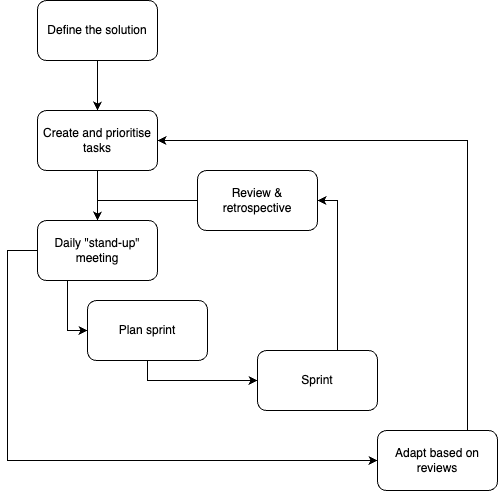
\includegraphics[width=0.6\textwidth]{Methodology diagram (1).png}
	\caption{- The stages of my methodology}
\end{figure}

\newpage

\subsection{A breakdown of each stage}

\begin{itemize}
    \item Define the solution: 
        Clearly outline the project's goals/objectives and identify the key features and functionalities the robot should possess. Break down the project into smaller, manageable tasks. This is the main part of my documentation: the analysis \& design stage.
    \item Create and prioritise tasks: prioritise the tasks based on their importance and urgency. Create a backlog of these prioritised tasks.

    \item Plan sprint: Divide the project into short, iterative development cycles (sprints). As a single developer, sprints will most likely take between a few hours and a few days. Select a subset of tasks from the backlog for each sprint.

    \item Conduct daily "stand-up" meetings with myself, noting what I accomplished the previous sprint, what I plan to do today, and any obstacles I face. This is essentially a "mini-review".

    \item Sprint: Focus solely on the tasks I assigned for the sprint; I will use the stand-up notes to ensure the backlog of tasks is cleared or allocated a time to be resolved.

    \item Review and retrospective: At the end of each sprint, I will review the completed tasks and assess progress, identifying any areas for improvement and adjusting my plan accordingly.

    \item Adapt and review: Once the backlog of each category of tasks is cleared, implement each section into the central program, regularly testing the code to ensure it meets the requirements. I will use version control systems (VCS) such as GitHub to track changes and document the problems I faced.
\end{itemize}

\subsection{Key considerations:}
\begin{itemize}
    \item Time Management: Effectively managing my time to ensure tasks are completed within the sprint time-frame.
    \item Communication: I plan to use tools like project management software or even a simple to-do list to track progress.
    \item Documentation: Using VCS, I aim to document any changes I make, as well as the reasons why.
\end{itemize}